% !TEX program = lualatex
% ECON 201, Worksheet 15: Supply and Demand.
% Compile with LuaLaTeX so the PDF is tagged. Build from the course root:
%   latexmk -lualatex -cd worksheets/worksheet15.tex && latexmk -c -cd worksheets/worksheet15.tex
% Every number here is computed and printed by slides/figures/make_lecture15.py
% (the homecoming ticket market, its own numbers rather than the deck's,
% read off the graph in figures/tickets.pdf, which the script also draws).
\DocumentMetadata{
  pdfstandard=UA-2,
  pdfversion=2.0,
  lang=en-US,
  tagging=on
}
\documentclass[11pt]{article}

\usepackage[letterpaper, margin=0.75in, top=0.5in, bottom=0.45in]{geometry}
\usepackage{fontspec}
\setmainfont{Fira Sans}
\usepackage{amsmath}
\usepackage{amssymb}
\usepackage{graphicx}
\usepackage{booktabs}
\usepackage{array}
\usepackage{xcolor}
\usepackage{needspace}
\usepackage[most]{tcolorbox}
\definecolor{cream}{HTML}{FDF3EA}
\definecolor{accent}{HTML}{BF5700}
\usepackage{titlesec}
\titleformat{\section}{\large\bfseries\color{accent}}{}{0pt}{}
\titlespacing*{\section}{0pt}{4pt}{2pt}
\usepackage{hyperref}
\hypersetup{pdftitle={ECON 201 Worksheet: Supply and Demand}, pdfauthor={Div Bhagia}, hidelinks}
\pagestyle{empty}
\setlength{\parindent}{0pt}
\setlength{\parskip}{2pt}

% Ruled answer space: n lines. Plain TeX loop; pgffor's \foreach breaks the
% enumerate counter when used inside an item.
\newcount\answerlinecount
\newcommand{\answerlines}[1]{%
  \par\vspace{1pt}\answerlinecount=#1
  \loop\ifnum\answerlinecount>0
    \rule{\linewidth}{0.3pt}\par\vspace{5pt}%
    \advance\answerlinecount by -1
  \repeat
  \vspace{-5pt}}

\begin{document}

{\LARGE\bfseries\color{accent} Worksheet: Supply and Demand}\hfill{\large ECON 201}

% Terms sit on the cream panel, where the brand orange falls below 4.5:1;
% the darker orange keeps WCAG AA contrast (see CLAUDE.md).
\definecolor{accentdark}{HTML}{8F4100}
\newcommand{\term}[1]{\textcolor{accentdark}{\textbf{#1}}}

% Definitions panel list: flush left, compact (see worksheet09).
\newenvironment{deflist}
  {\begin{list}{\textbullet}{%
     \setlength{\leftmargin}{1.1em}\setlength{\labelwidth}{0.7em}%
     \setlength{\labelsep}{0.4em}\setlength{\itemindent}{0pt}%
     \setlength{\listparindent}{0pt}\setlength{\topsep}{2pt}%
     \setlength{\partopsep}{0pt}\setlength{\parsep}{0pt}%
     \setlength{\itemsep}{2pt}}}
  {\end{list}}

\begin{tcolorbox}[colback=cream, colframe=accent, boxrule=0.6pt, arc=2pt,
  left=6pt, right=6pt, top=4pt, bottom=4pt, title=Definitions,
  fonttitle=\bfseries, coltitle=white]
\begin{deflist}
\item \term{Demand curve}: how many units buyers want to buy at each price.
\item \term{Supply curve}: how many units sellers want to sell at each price.
\item \term{Market-clearing price}, or equivalently the \term{equilibrium price}:
  the price at which the quantity demanded equals the quantity supplied. The
  quantity traded at that price is the \term{equilibrium quantity}.
\item \term{Excess demand}: the quantity demanded is greater than the quantity
  supplied at the current price. \term{Excess supply}: the quantity supplied is
  greater than the quantity demanded at the current price.
\end{deflist}
\end{tcolorbox}

\needspace{5\baselineskip}\section{The homecoming game}

Students resell tickets to the homecoming game to each other. The graph shows
the demand curve of the students who want a ticket and the supply curve of the
students who have one to sell.

\begin{center}
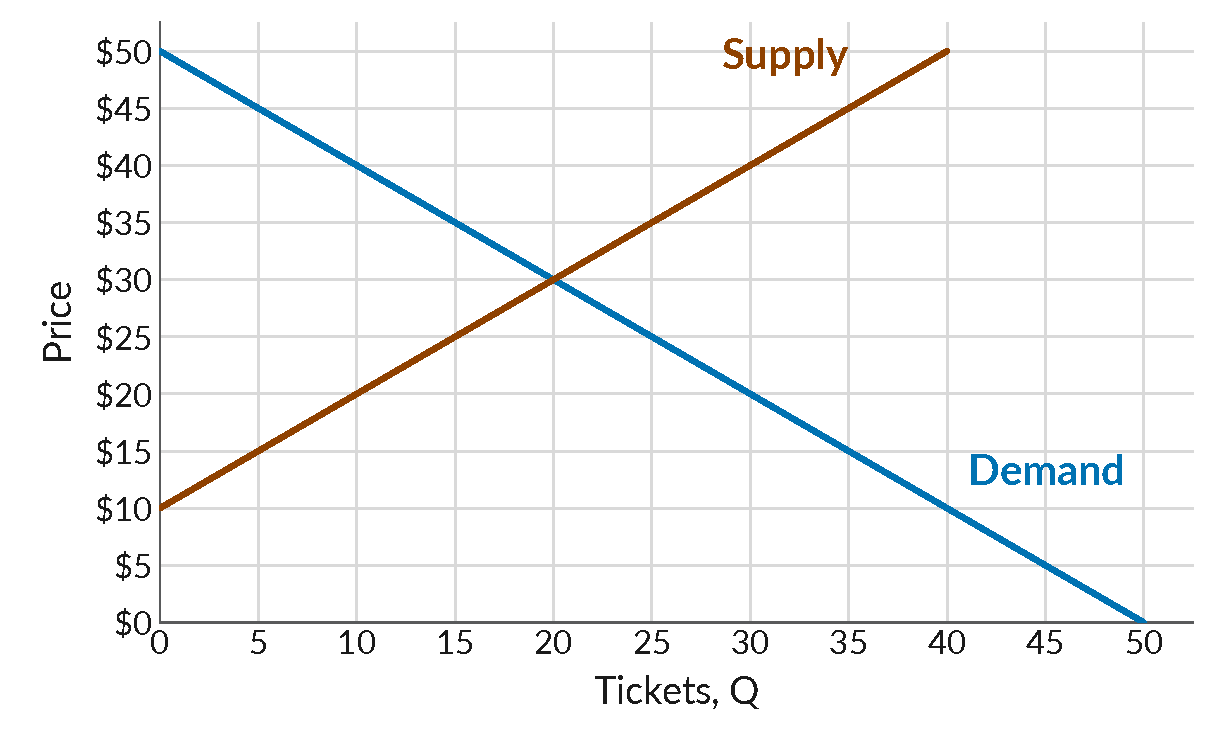
\includegraphics[width=0.6\textwidth, alt={A plotting grid, price on the
vertical axis from 0 to 50 dollars with gridlines every 5 dollars, and tickets
on the horizontal axis from 0 to 50 with gridlines every 5 tickets. The demand
curve falls in a straight line from 50 dollars at zero tickets to zero at 50
tickets. The supply curve rises in a straight line from 10 dollars at zero
tickets to 50 dollars at 40 tickets. They cross at 20 tickets and 30 dollars.}]{figures/tickets.pdf}
\end{center}

\vspace{4pt}
1. What is the quantity demanded at a price of \$20? What is the quantity
supplied?
\answerlines{1}

2. At \$20, is there an excess demand or an excess supply? If so, by how much?
\answerlines{1}

3. At \$20, would it make sense for some buyers to change what they do? What
about sellers? Which way does the price move?
\answerlines{2}

4. What are the equilibrium price and quantity in this market? Mark the point
on the graph.
\answerlines{1}

5. Suppose the price were \$40 instead. Is there an excess demand or an excess
supply, and by how much? Which way does the price move?
\answerlines{2}

\end{document}
